

\section{Approach}
\label{sec:approach}

The target of our method is to recover the missing contents in a corrupted video with fine details and temporal consistence.
%
%Our intuition is that there exists complementary information in neighboring frames, which can benefit the inpainting process of each individual frame.Therefore, 
In each inference batch to fill up the missing part in frame $X_t$, total $T$ frames $\boldsymbol{X}$ ($T=5$), indexed by $\msset{X}$, are fed to our inpainting network, as well as the corresponding masks $\boldsymbol{M}$ that indicate the missing regions.
The final output is the completed frame \(Y_t\) at time $t$. 
%Our method infers each target frame $Y_t$ individually but with hints from its neighboring source frames.
%To fill up the missing region with structural details and temporal coherence, 
As Fig.~\ref{fig:stiNet} shows, our network consists of two paths. 
The first is an edge-guided inpainting path, which consists of an edge inpainting network ENet that recovers missing edges of the input frames, a coarse-to-fine texture inpainting network TexNet that replenishes appearance details under the structure guidance.
The second path leverages motion flows to enhance temporal coherence of the completed frames.
It consists of a flow inpainting network FNet that predicts the motion flows in the missing regions and an ensemble module that aggregates previously synthesized frames to refine the current frame. 



\subsection{Edge Inpainting Network}
\label{sec:edgenet}
 
To fill the missing regions with fine details, their corresponding structural edges are predicted, and provide structural guidance for the following texture synthesis.
%
Given the input corrupted frames $\boldsymbol{X}$, a canny edge detector is first used to extract the edge maps $\boldsymbol{E}^{i}$. %Notably, the edges in the masked regions in $\boldsymbol{E}^{i}$ are missed. 
%Given the incompleted grayscale images $\boldsymbol{X}^{g}$ of input frame, a canny edge detector is first used to generate initial edge maps . 
Then, the ENet completes the missing edges.
The input of ENet consists of the grayscale frames $\boldsymbol{X}^{g}$, initial edge maps $\boldsymbol{E}^{i}$, and their corresponding masks $\boldsymbol{M}$.
%
As shown in Fig.~\ref{fig:stiNet}, ENet consists of a generator $G^E$ and a discriminator $D^E$.
$G^E$ is composed of a two-layer 3D encoder, eight 2D residual blocks, and a two-layer 3D decoder. 
The 3D encoder and decoder are designed to learn the spatio-temporal correlation, while the 2D residual blocks are used to enrich spatial features in larger receptive fields. The discriminator $D^E$ follows the $70\times 70$ PatchGAN architecture \cite{Isola_2017_CVPR}. 
Finally, the inpainted edge maps are obtained by:
\begin{equation}
\label{eq:edgenet}
\boldsymbol{E}=G^E(\boldsymbol{E}^{i},\boldsymbol{X}^{g},\boldsymbol{M}).
\end{equation}

The ENet is trained by playing a minimax game to optimize the generator $G^E$ and the discriminator $D^E$ as
\begin{equation}
\label{eq:loss_e}
\mathcal{O}_{edge} =\min\limits_{G^E} \max \limits_{D^E} \big(\mathcal{L}^E_{adv}+\lambda_1 * \mathcal{L}^E_{fm}\big),
\end{equation}
where $\mathcal{L}^E_{adv}$ and $\mathcal{L}^E_{fm}$ are the adversarial loss and feature matching loss. 
$\lambda_1$ is a hyper-parameter to balance the three terms.
%
Following the adversarial learning manner, $\mathcal{L}^E_{adv}$ can facilitate ENet to produce plausible edge maps by:
\begin{equation} \label{eq:edge_adver}
\begin{aligned} 
\mathcal{L}^E_{adv}  =&\mathbb{E}_{(\boldsymbol{E}^{gt},\boldsymbol{X}^{g})}\big[logD^E(\boldsymbol{E}^{gt},\boldsymbol{X}^{g})\big]\\ 
+&\mathbb{E}_{(\boldsymbol{E},\boldsymbol{X}^{g})}\big[log\big(1-D^E ( \boldsymbol{E},\boldsymbol{X}^{g})\big)\big],
\end{aligned}
\end{equation}
where $\boldsymbol{E}^{gt}$ represents the ground truth edge maps. $\mathcal{L}^E_{fm}$ evaluates the feature-level similarity between ground truth edge maps and predicted edge maps, which helps to create structurally rational edge maps. 
Feature matching loss was first proposed in \cite{wang2018high} and has been widely used in recent GANs.
The feature matching loss is defined as:
\begin{equation}
\label{eq:edge_fm}
\mathcal{L}^E_{fm}=\sum_{k=1}^L{\frac{1}{N_k}\left\| D^E_k(\boldsymbol{E}^{gt},\boldsymbol{X}^{g})- D^E_k(\boldsymbol{E},\boldsymbol{X}^{g})\right\|_1},
\end{equation}
where $D^E_k$ is the output of the $k$-th layer in $D^E$, while $N_k$ is the element number of $D^E_k$. 
%Note that the discriminator $D^E$ is not optimized by the feature matching loss term. It plays as a feature extractor to optimize the generator $G^E$ for producing plausible edge maps $\boldsymbol{E}$.


\begin{figure}[t]
	\centering
	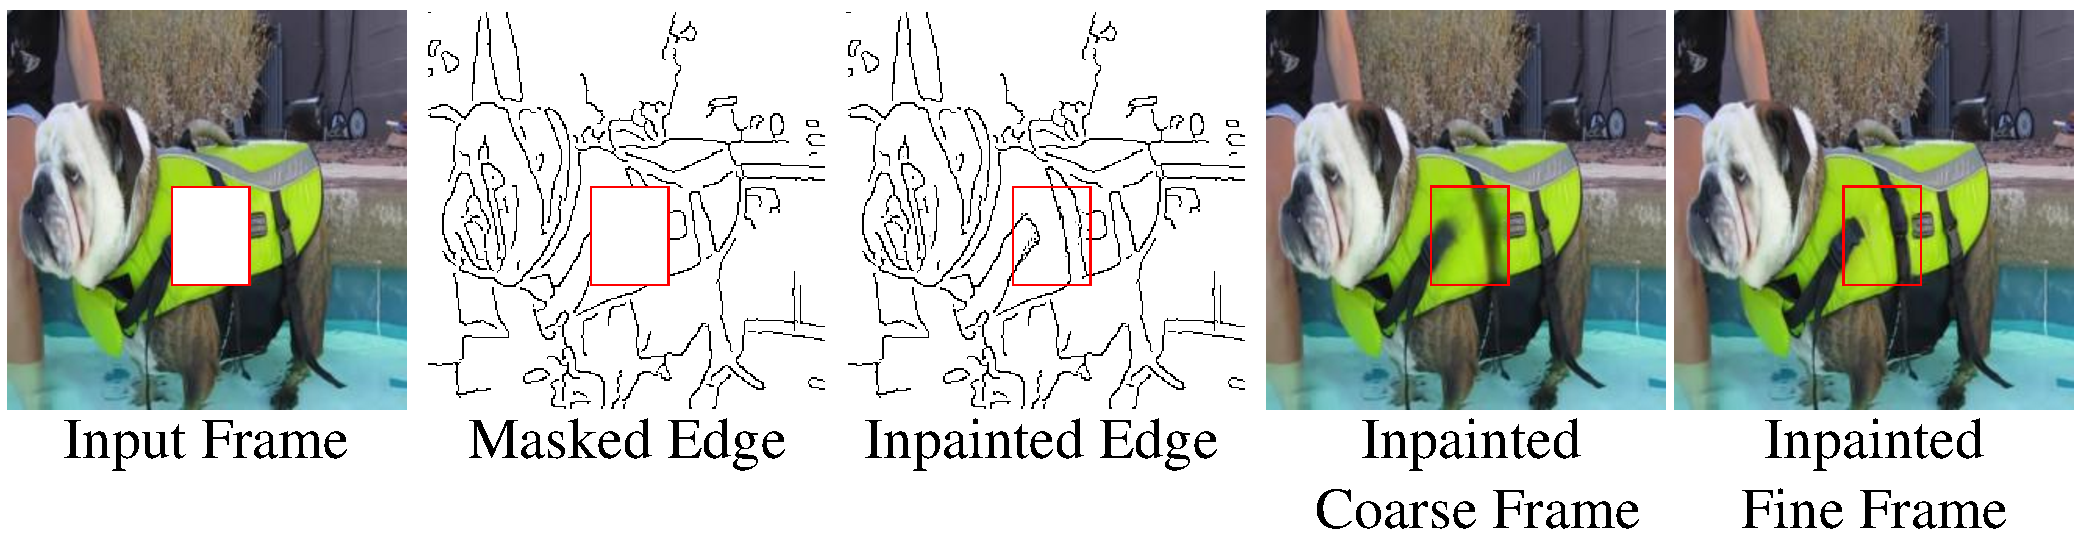
\includegraphics[width=1.0\columnwidth]{coars-fine} % Reduce the figure size so that it is slightly narrower than the column. Don't use precise values for figure width.This setup will avoid overfull boxes. 
	\caption{Given a corrupted frame (a), our ENet first completes sparse edges (b) which well represent the structure of the missing content. Then TexNet progressively replenishes textures under the guidance of synthesized edges from coarse (c) to fine (d).}
	
	\label{fig:coarse-fine}
\end{figure}



\subsection{Edge-Guided Texture Inpainting Network}

%Combining the inpainted edge maps $\boldsymbol{E}$ and flow maps $\boldsymbol{O}$, a spatio-temporal inpainting network (STINet) is designed to obtain the final target frame $Y_t$.

Given the completed edge maps $\boldsymbol{E}$ for the 
$T$ frames, then we fill textures under the structural guidance in a coarse-to-fine manner. 
%
The proposed TexNet consists of a coarse network and a refinement network, as Fig.~\ref{fig:stiNet} shows.
%
The input of TexNet is the concatenation of $\boldsymbol{X}$, $\boldsymbol{E}$, and $\boldsymbol{M}$.
First, the coarse inpainting network consists of a set of 3D convolutions to capture the temporal information, which targets to produce an rough completion for the $T$ frames  $\boldsymbol{Y}^i$ with colors.
%The 3D coarse network incorporates neighboring frames by convolutions of the time dimension.
Second, the refinement network takes the synthesized edge maps $\boldsymbol{E}$, $\boldsymbol{Y}^i$ and $\boldsymbol{M}$ as input and uses 2D convolutions to enhance structure details and synthesize frame $Y^T_t$. 
%For the corrupted region, our ENet first completes sparse edges which well represent the structure of the missing content, then TexNet progressively replenishes textures under the guidance of synthesized edges.



To fully exploit the structural information in $\boldsymbol{E}$, we design a structure attention module (SAM) in the refinement network.
The core insight of the SAM is to capture the spatial correlation between edges and textures.
The detailed implementation of the SAM is given in Fig.~\ref{SEM}.
%Two separate convolution blocks are first applied to embed structure features from the predicted edge maps $\boldsymbol{E}$.
% which alleviate the feature discrepancy between structural edge and video texture.
The intermediate video features and embedded edge features are interacted to calculate the latent structure-texture correlation via matrix multiplication. 
%After a SoftMax operation, the normalized attention map represents long-range correlation between the structure and high-level video features.
%
The normalized attention map is applied to the intermediate video features, and the structure information is thus embedded in TexNet.
After introducing structural guidance, the inpainted content by TexNet becomes more structurally and semantically realistic, as Fig.~\ref{fig:coarse-fine} shows.
%Fig.~\ref{fig:coarse-fine} shows an example of our structure-guided inpainting result. 
 


To train the TexNet, we define the loss function as:
%
\begin{equation}
	\label{eq:1}
		\mathcal{O}_{tex}=\min\limits_{G^T} \max \limits_{D^T} \big(\mathcal{L}^{T}_{rec}+\mathcal{L}^T_{adv}\big).
\end{equation}
%
Inspired by \cite{nazeri2019edgeconnect}, the first term $\mathcal{L}^{T}_{rec}$ is the $l_1$-reconstruction loss to measure the difference between predicted video frames and the ground truth video frames $\widetilde{\boldsymbol{Y}}$.
Different from \cite{nazeri2019edgeconnect}, we penalize both the coarse predictions $\boldsymbol{Y}^i$ and refined frame $Y^{T}_t$, given by:
\begin{equation}
	\begin{aligned}
		\mathcal{L}^{T}_{rec}&=\frac{1}{\left\|\boldsymbol{M} \right\|_1}\left\|(\boldsymbol{Y}^i-\widetilde{\boldsymbol{Y}})\odot \boldsymbol{M}\right\|_1\\ &+\lambda_2*\frac{1}{\left\|M_t \right\|_1}\left\|(Y^T_t-\widetilde{Y}_t)\odot M_t\right\|_1.
	\end{aligned}
\end{equation}
%
%
Besides, an extra adversarial loss $\mathcal{L}^T_{adv}$ is introduced to promote the visual realism of the generated frame.
\dlt{ by:
%$\mathcal{L}^I_{adv}$ is defined as:
\begin{equation}
	\label{eq:inp_adver}
	\mathcal{L}^I_{adv}=\mathbb{E}[logD^I(\widetilde{Y}_t)]+\mathbb{E}[log\big(1-D^I(Y^I_{t})\big)],
\end{equation}
where $G^I$ is the TexNet and $D^I$ has the similar architecture with $D^E$.}
% $\mathcal{L}^I_{adv}$ enforces the generated frame to be more realistic.





 \begin{figure}[t]
	\centering
	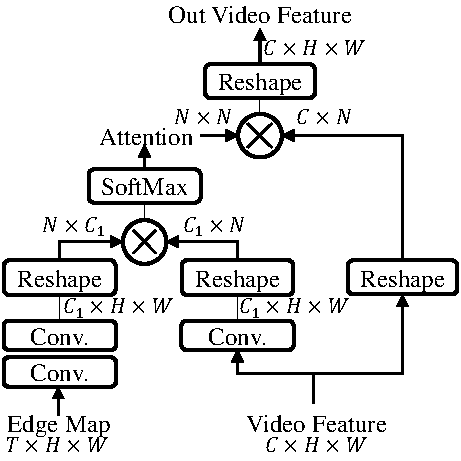
\includegraphics[width=0.7\columnwidth]{SEM} % Reduce the figure size so that it is slightly narrower than the column. Don't use precise values for figure width.This setup will avoid overfull boxes. 
	\caption{Architecture of the structure attention module. $C$ is the channel of the input video features, and $N=H\times W$. $\otimes$ represents matrix multiplication. Usually, we set $C_1=C/8$.}
	\label{SEM}
\end{figure} 


\begin{table*}[t]
	\caption{Comparisons with existing methods on YouTubeVOS. To save space, the year of method is not listed.}\smallskip
	
	\centering
	\resizebox{2.0\columnwidth}{!}{
		\smallskip\begin{tabular}{c|c|c|c|c|c|c|c|c|c|c }
			\hline
			&\multicolumn{3}{c|}{Fixed Square Mask}& \multicolumn{3}{c|}{Moving Square Mask}&\multicolumn{3}{c|}{Free-Form Mask}&Inference \\
			\cline{2-10} 
			&PSNR & SSIM & FID & PSNR & SSIM & FID & PSNR & SSIM & FID&Speed(fps))\\
			\hline
			Nazeri et al. &28.6446 &0.9484  &   38.2116  &	
			30.7478 & 0.9647 &  16.2739  &
			25.6693  & 0.9088 &  43.0366&22.81 \\
			\hline
			Wang et al. &27.9668 & 0.9515 &  40.7199  &	 
			31.5776	& 0.9678 &  13.8383&   
			32.1862 & 0.9626 & 19.1191 &8.1634 \\
			\hline
			
			
			Kim et al. b& 28.0846&0.9468 &  39.9377  & 
			36.8598	& 0.9728 &7.2315  &
			33.5549	& 0.9646 & 9.3797&1.2275  \\
			\hline
			Xu et al. &29.0531 & 0.9497 &  32.8860  & 
			37.8241& 0.9772 &6.3746  &
			32.6287 &0.9618  &  11.1501&0.5620 \\
			\hline
			
			\hline
			
			
			TexNet &28.0174 &0.9494  &  42.7164   &	
			33.8131 &  0.9705  &8.2390	& 
			30.0680& 0.9390 & 20.6358&7.6335
			\\
			\hline
			+edge input  &29.5242 &  0.9520& 36.2097   &	
			37.6630	& 0.9798 &3.5161    &	
			33.8206	&0.9659  &    6.6651& 5.2356 \\
			\hline
			
			+SAM &29.9918 &  0.9533 &  27.4198  &	
			38.2433	& 0.9807 &   2.5083  &	
			35.7783	&0.9712  &   5.8786 & 5.1546\\
			\hline
			
			
			
			
			Ours &\textbf{30.0590} &\textbf{0.9543}&   \textbf{27.2431} &
			\textbf{38.8186} & \textbf{0.9824} & \textbf{2.3455} &
			\textbf{35.9613}  & \textbf{0.9721}&  \textbf{ 5.8694} &2.5643\\
			
			\hline
			
			
		\end{tabular}
	}
	\label{tab:sem}
\end{table*}







\subsection{Flow-Guided Temporal Coherence Enhancement}
\label{sec:fec}
It is vital to maintain temporal consistency in video inpainting.
%Optical flows are widely used to represent the dense correspondence between frames.
To enhance temporal consistency in the synthesized results, we employ optical flows to smooth the inpainted edge maps and synthesized frames from ENet and TexNet.
% and reinforce the temporal coherence between neighboring edge maps and frames during training. 
Moreover, we design an ensemble module which leverages the previous inpainted frames to refine the current frame completion, as Fig.~\ref{fig:stiNet} shows. 
%
We design a flow inpainting network (FNet) to predict the optical flow in the missing region.
%
Similar to ENet, a set of initial flow maps \(\boldsymbol{O}^i\) for pairs between the current frame $X_t$ and its neighboring frames are first generated using a flow extraction network, such as FlowNet2.0~\cite{Flownet_2017_CVPR}.
Notably, \(\boldsymbol{O}^i\) consists of four flow maps \((O^i_{t\Rightarrow t-7}, O^i_{t\Rightarrow t-3}, O^i_{t\Rightarrow t+3}, O^i_{t\Rightarrow t+7})\).
From the predicted optical flows $\boldsymbol{O}^i$, FNet estimates the flows in the missing regions to obtain four flow maps \(\boldsymbol{O}\) as:
\begin{equation}
	\label{eq:flownet}
	\boldsymbol{O}=G^F(\boldsymbol{O}^{i},\boldsymbol{M}),
\end{equation}
where $G^F$ denotes FNet, which consists of an encoder that uses ResNet101 \cite{He_2016_CVPR} as backbone and a decoder.
%The detailed architecture of FNet is shown in Fig.~\ref{fig:stiNet}.

To train the flow inpainting network, the loss function is given by:
\begin{equation}
	\label{eq:flow_all}
	\mathcal{O}_{flow}=\min\limits_{G^F} \big(\mathcal{L}^F_{rec}+ \mathcal{L}^F_{har}+\mathcal{L}_{fec}\big),
\end{equation}
where $\mathcal{L}^F_{rec}$ and $\mathcal{L}^F_{har}$ are respectively $l_1$ loss and hard example mining loss in the missing regions, following the definition in \cite{Xu_2019_CVPR}. 
%Specifically, $\mathcal{L}^F_{har}$ encourages the network to focus on those hard samples in order to avoid blurry texture.




To enhance temporal consistency in the synthesized results, we apply the completed flows to warp the inpainted edge maps and compute the consistency between neighboring edge maps. 
%
Instead of separately training two subnetworks ENet and FNet, we train them jointly, because the temporal correlation and structural details can boost each other. 
To achieve this goal, a flow-edge consistency loss is defined as:
%
\begin{equation}
	\label{eq:flow_edge}
	\mathcal{L}_{fec}=\sum_{k}\frac{1}{\left\|M_{t} \right\|_1}\left\|(E_{t}-\phi(O_{t\Rightarrow t-k},E_{t-k}))\odot M_{t}\right\|_1,
\end{equation}
where $\phi(O_{t\Rightarrow t-k},E_{t-k})$ is the warping operation which warps the edge map $E_{t-k}$ to the target frame according to the generated optical flow $O_{t\Rightarrow t-k}$.
$k$ denotes the index of neighboring frames ($k\in \left\{-7,-3,+3,+7 \right\}$). Also, $\mathcal{L}_{fec}$ is added to Eq.~\eqref{eq:loss_e} for joint training of ENet and FNet.
%Specifically, $\mathcal{L}_{fec}$ warps the edge maps from neighboring frames to the target frame to penalize the reconstruction loss.
%In terms of ENet, $\mathcal{L}_{fec}$ encourages the predicted edge maps to be temporally smoothing, which should conform to the motion tendency in the flow maps $\boldsymbol{O}$. 
%In terms of FNet, $\mathcal{L}_{fec}$ constrains the model to focus on edges.
%Thus, the total loss function for joint training of ENet and FNet is:
%\begin{equation}
%	\label{eq:flow}
%	\mathcal{L}_{joint}=\mathcal{L}_{edge}+\mathcal{L}_{flow}+ \mathcal{L}_{fec}.
%\end{equation}


To eliminate temporal flickers in the completed video frames, we enforce the temporal coherence of synthesized neighboring frames via a flow warping constraint $\mathcal{L}^T_{flo}$. 
%
Specifically, the neighboring frames are warped into the target frame to compute the difference: 
\begin{equation}
\label{eq:inp_flow}
\mathcal{L}^T_{flo}=\sum_{\widehat{t}\in\mathcal{T}}\left\| Y^T_t-\phi(O_{t\Rightarrow \widehat{t}},Y_{\widehat{t}}) \right\|_1,
\end{equation}
where $\mathcal{T}=\{t-7,t-3\}$. $\phi(O_{t\Rightarrow \widehat{t}},Y_{\widehat{t}})$ warps $Y_{\widehat{t}}$ to $Y^T_{t}$ using flow $O_{t\Rightarrow \widehat{t}}$.
%$O_{t\Rightarrow \widehat{t}}$ is predicted using the subsequent flow inpainting network.
%$\mathcal{L}^I_{flo}$ expects that all the neighboring frames can be well warped to the target frame with small reconstruction loss.
%
$\mathcal{L}^T_{flo}$ is added to Eq.~\eqref{eq:1}.
Finally, a temporal ensemble module is designed 
to refine the current frame $Y_t$ by aggregating previous frames. %The architecture is shown in Fig.~\ref{fig:stiNet}. 
This module is trained with a $l_1$-reconstruction loss and an adversarial loss.







